\documentclass{article}
\usepackage{stackengine}
%\usepackage[utf8]{inputenc}
\usepackage[T1]{fontenc}
\usepackage{amsmath}
\usepackage{amsfonts}
\usepackage{graphicx}
\usepackage{pbsi}
\usepackage{lmodern}
%\usepackage{tgbonum}
\usepackage[a4paper]{geometry}
\usepackage{pdflscape}
\usepackage[dvipsnames, svgnames]{xcolor}
\usepackage[pages=some]{background}
\usepackage{tikz}
\usetikzlibrary{math} 
\usetikzlibrary{automata,positioning}
\usetikzlibrary[decorations.text]
\usetikzlibrary{arrows.meta} % LATEX and plain TEX when using Tik Z
%\usetikzlibrary[automata]
\usetikzlibrary{calc}

\newcommand\BackImage[2][scale=1]{%
\BgThispage
\backgroundsetup{
scale=1,
angle=0,
opacity=1,  %% adjust
contents={\includegraphics[width=\paperwidth,height=\paperheight]{#2}}
%contents={\includegraphics[#1]{#2}}
}
}

\newcommand*{\vertchar}[2][0pt]{%
  \tikz[
    inner sep=1pt,
    shorten >=-.15ex,
    shorten <=-.15ex,
    line cap=round,
    baseline=(c.base),
  ]\draw
    (0,0) node (c) {#2}
    ($(c.north)+(#1,0)$) -- ($(c.north)+(#1,0)$);%
}


\makeatletter
\newcommand{\dotr}[1]{%
  \mathpalette\@dotr{#1}%
}

\newcommand*{\@dotr}[2]{%
  % #1: math style (\displaystyle, ..., \scriptscriptstyle)
  % #2: argument of \dotr
  \sbox0{$\m@th#1#2$}%
  \usebox{0}%
  % simulating a superscript
  %\raisebox{\dimexpr\ht0-\height}{$\m@th#1\addvbuffer[-1ex 0.9ex]{.}}%
  \raisebox{3.5pt}{$\m@th#1\@smallbullet#1\bullet$}%
  \kern\scriptspace
}
\newcommand*{\@smallbullet}[2]{%
  \scalebox{.3}{$\m@th#1#2$}%
}
\makeatother
    
\newcommand*{\siin}[1]{\stackinset{c}{}{b}{5.5pt}{\small\ttfamily\char'15}{#1}}
\newcommand*{\nn}{\textsuperscript{n}}

\newcommand*{\pehin}[1]{\stackinset{c}{}{b}{5.5pt}{\small\ttfamily\char'15}{#1}}
\newcommand*{\dtr}{\raisebox{3.5pt}{$\scalebox{.3}{$\bullet$}$}}
\newcommand*{\dtrh}{\raisebox{5pt}{$\scalebox{.3}{$\bullet$}$}}



\begin{document}

\hspace*{-30mm}
\resizebox{18cm}{!} {
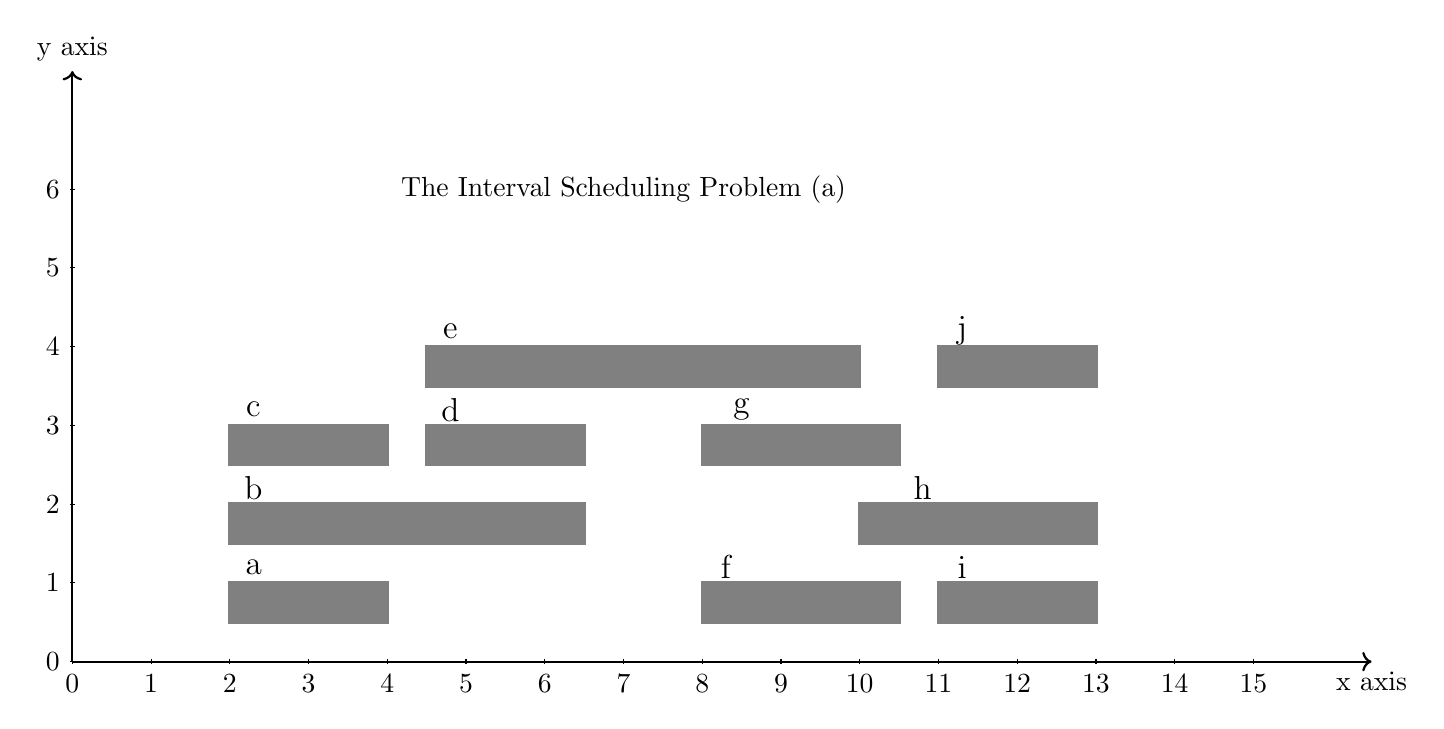
\begin{tikzpicture} 

\foreach \x in {0,1,2,3,4,5,6,7,8,9,10,11,12,13,14,15}
   \draw (\x cm,1pt) -- (\x cm,-1pt) node[anchor=north] {$\x$};
\foreach \y in {0,1,2,3,4,5,6 }
    \draw (1pt,\y cm) -- (-1pt,\y cm) node[anchor=east] {$\y$};
\draw[thick,->] (0,0) -- (16.5,0) node [anchor= north]{x axis};
\draw[thick,->] (0,0) -- (0,7.5) node [anchor= south] {y axis};


\filldraw [gray, very thick] (2,0.5) -- (2,1) -- (4,1) -- (4,0.5) -- cycle ;
\filldraw [gray, very thick] (8,0.5) -- (8,1) -- (10.5,1) -- (10.5,0.5) -- cycle ;
\filldraw [gray, very thick] (11,0.5) -- (11,1) -- (13,1) -- (13,0.5) -- cycle ;
\filldraw [gray, very thick] (2,1.5) -- (2,2) -- (6.5,2) -- (6.5,1.5) -- cycle ;
\filldraw [gray, very thick] (10,1.5) -- (10,2) -- (13,2) -- (13,1.5) -- cycle ;
\filldraw [gray, very thick] (2,2.5) -- (2,3) -- (4,3) -- (4,2.5) -- cycle ;
\filldraw [gray, very thick] (4.5,2.5) -- (4.5,3) -- (6.5,3) -- (6.5,2.5) -- cycle ;
\filldraw [gray, very thick] (8,2.5) -- (8,3) -- (10.5,3) -- (10.5,2.5) -- cycle ;
\filldraw [gray, very thick] (4.5,3.5) -- (4.5,4) -- (10,4) -- (10,3.5) -- cycle ;
\filldraw [gray, very thick] (11,3.5) -- (11,4) -- (13,4) -- (13,3.5) -- cycle ;


\path 
(2.3,1.2) node{\large a} 
(8.3, 1.2) node {\large f}
(11.3, 1.2) node {\large i}
(2.3, 2.2) node {\large b}
(10.8, 2.2) node {\large h}
(2.3,3.2) node {\large c}
(4.8,3.2) node {\large d}
(8.5,3.2) node {\large g}
(4.8,4.2) node {\large e}
(11.3,4.2) node {\large j};

\draw (7,6) node {The Interval Scheduling Problem (a)};

\end{tikzpicture}
}
\vspace*{5mm} \newline
\hspace*{-25mm}
\resizebox{18cm}{!} {
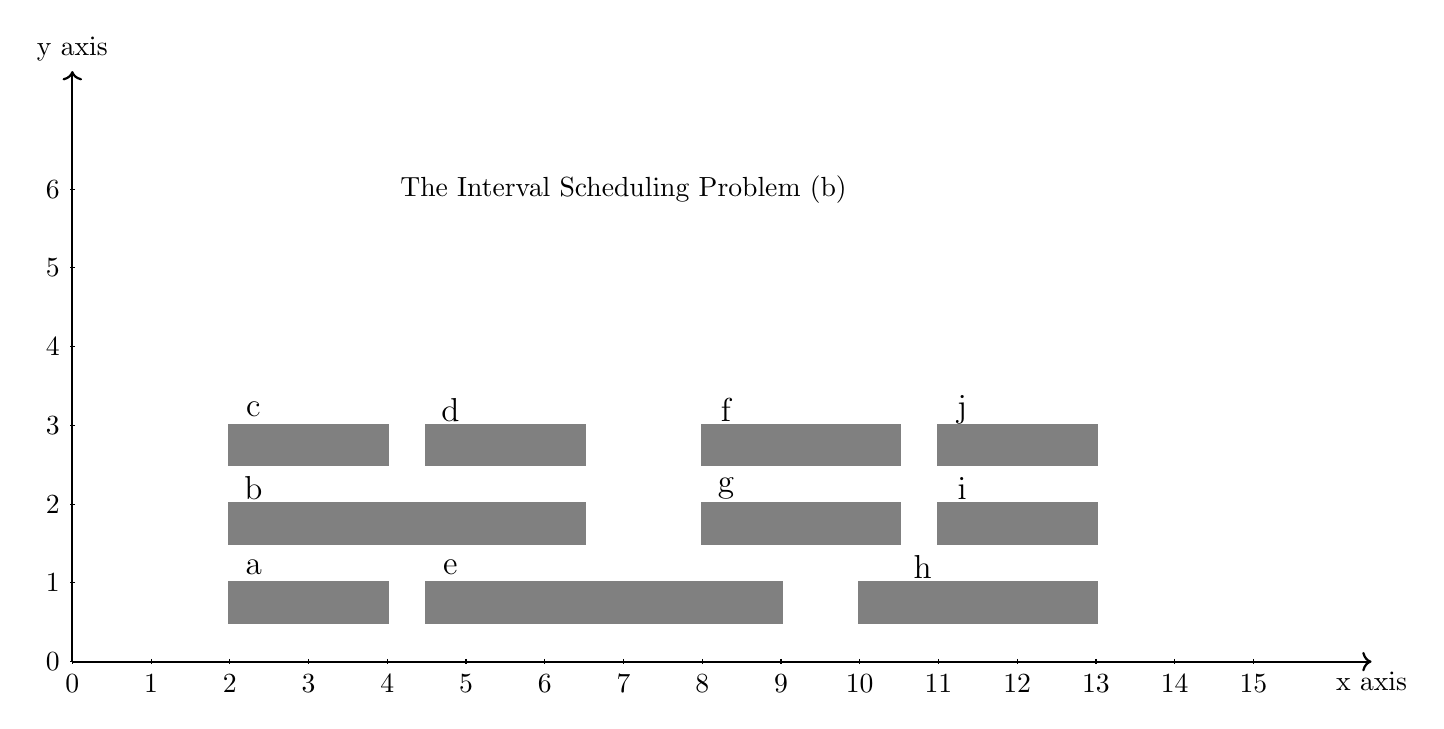
\begin{tikzpicture} 

\foreach \x in {0,1,2,3,4,5,6,7,8,9,10,11,12,13,14,15}
   \draw (\x cm,1pt) -- (\x cm,-1pt) node[anchor=north] {$\x$};
\foreach \y in {0,1,2,3,4,5,6 }
    \draw (1pt,\y cm) -- (-1pt,\y cm) node[anchor=east] {$\y$};
\draw[thick,->] (0,0) -- (16.5,0) node [anchor= north]{x axis};
\draw[thick,->] (0,0) -- (0,7.5) node [anchor= south] {y axis};

\filldraw [gray, very thick] (2,0.5) -- (2,1) -- (4,1) -- (4,0.5) -- cycle ;
\filldraw [gray, very thick] (4.5,0.5) -- (4.5,1) -- (9,1) -- (9,0.5) -- cycle ;
\filldraw [gray, very thick] (10,0.5) -- (10,1) -- (13,1) -- (13,0.5) -- cycle ;
\filldraw [gray, very thick] (2,1.5) -- (2,2) -- (6.5,2) -- (6.5,1.5) -- cycle ;
\filldraw [gray, very thick] (8,1.5) -- (8,2) -- (10.5,2) -- (10.5,1.5) -- cycle ;
\filldraw [gray, very thick] (11,1.5) -- (11,2) -- (13,2) -- (13,1.5) -- cycle ;
\filldraw [gray, very thick] (2,2.5) -- (2,3) -- (4,3) -- (4,2.5) -- cycle ;
\filldraw [gray, very thick] (4.5,2.5) -- (4.5,3) -- (6.5,3) -- (6.5,2.5) -- cycle ;
\filldraw [gray, very thick] (8,2.5) -- (8,3) -- (10.5,3) -- (10.5,2.5) -- cycle ;
\filldraw [gray, very thick] (11,2.5) -- (11,3) -- (13,3) -- (13,2.5) -- cycle ;


\path 
(2.3,1.2) node{\large a} 
(8.3, 3.2) node {\large f}
(11.3, 2.2) node {\large i}
(2.3, 2.2) node {\large b}
(10.8, 1.2) node {\large h}
(2.3,3.2) node {\large c}
(4.8,3.2) node {\large d}
(8.3,2.2) node {\large g}
(4.8,1.2) node {\large e}
(11.3,3.2) node {\large j};

\draw (7,6) node {The Interval Scheduling Problem (b)};

\end{tikzpicture}
}
\end{document}